

We study the public Wi-Fi characteristics using the traces collected 
from a shopping mall. 
The traces are collected in a coffee shop at Saturday 4pm. 

\subsection{Data Collection}

We create a monitor interface on a laptop and use \emph{libpcap}
library to capture the Wi-Fi data packets. 
We capture data packets from three channels in 2.4GHz 
(with center frequency 2412MHz, 2437MHz and 2462MHz) and
three channels from 5GHz (with center frequency 5180MHz, 5200MHz and 5220MHz), respectively. 
We collect 20 mins data traces from each channel. 
We repeat the same process in an apartment in a 
resident area and an office environments. 

\subsection{AP RSSI}

\begin{figure}[!ht]
 \centering
    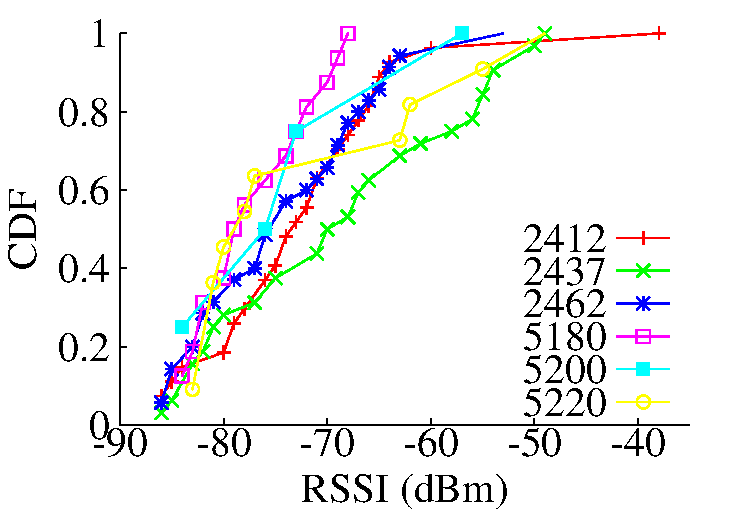
\includegraphics[width=0.5\textwidth]{./figures/public_ap_rssi}
 \caption{The RSSI distribution of public Wi-Fi APs.}
  \label{fig:public_ap_rssi}
\end{figure}



\subsection{Medium Utilization}

\begin{figure}[!ht]
 \centering
    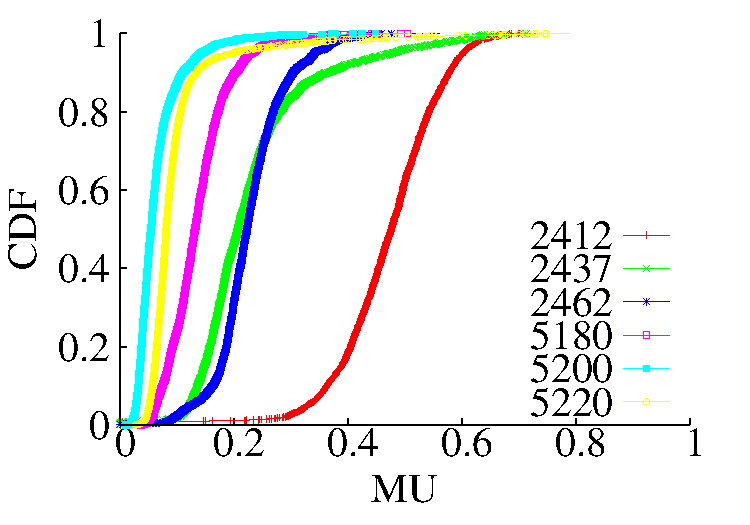
\includegraphics[width=0.44\textwidth]{./figures/public_mu_raw}
    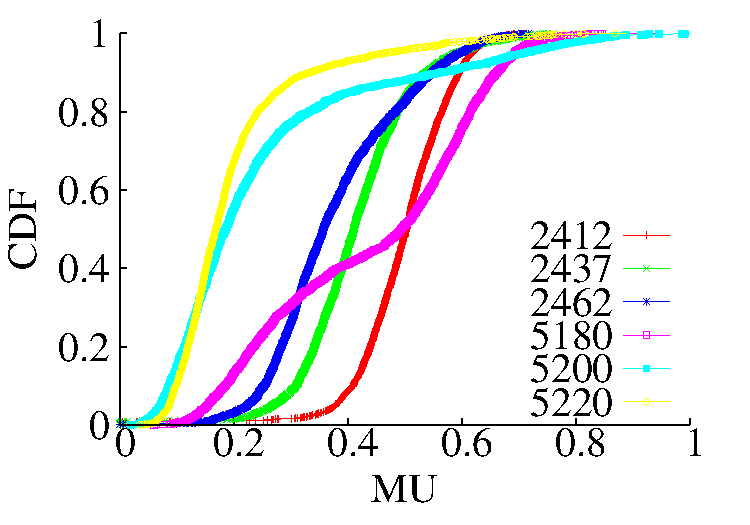
\includegraphics[width=0.44\textwidth]{./figures/public_mu_estimated}
 \caption{The Medium Utilization (MU) of public Wi-Fi.}
  \label{fig:public_mu}
\end{figure}




